We conduct acoustical measurements in a $3.6 \times 2.35 \times 2.55$~m ($l \times w \times h$) anechoic chamber with 8-inch deep (equal to $1/4$ wavelength at $\sim425$~Hz) anechoic foam wedges.
In the chamber, we place a circular arc which stands vertically and is aligned to be concentric with the ``origin'' of the chamber (i.e., where the center of the subject's head is ultimately placed). 
We attach to the arc eight loudspeakers (Genelec 8030A), which are equally-spaced (in $15^\circ$ increments) between $-30^\circ$ and $75^\circ$ elevation, and we include a ninth loudspeaker mounted on a separate stand at $-57^\circ$ elevation.\footnote{Here, we use the same spherical coordinate system as that defined in \citet{AES69-2015}.}
Specifically, we align the high-frequency drivers of the loudspeakers with these elevations such that the distance from each high-frequency driver to the origin is approximately $0.76 \pm 0.005$~m.
We also place, directly below the origin, a custom-built chair that is affixed to a computer-controlled turntable (Outline ET250-3D), whose axis of rotation passes through the origin of the chamber.
The chair, which is designed to have a minimal effect on incident acoustic waves,
consists of a drum-throne seat with backrest and a thin ``headrest'' structure that provides a reference for positioning the subject's head,
in order to minimize head movements during measurements.
An image of the setup is shown in \figref{fig:HRTF_setup}.

\begin{figure}[t]
\begin{center}
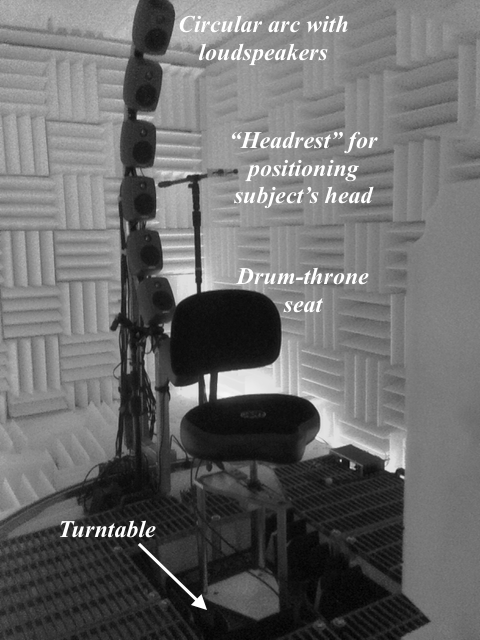
\includegraphics[width = 0.7\textwidth]{a4_HRTF_measurements/figures/HRTF_setup.png}
\caption{Setup used to make HRTF measurements.}.
\label{fig:HRTF_setup}
\end{center}
\end{figure}

Prior to making measurements, we calibrate and equalize the binaural microphones (Theoretica Applied Physics BACCH-BM Pro).
We first adjust, for each channel, the microphone gain (using a B\&K Type 4231 calibrator and DP-0978 adapter) such that a 94~dBSPL (rms) sine tone produces a $-11$~dBFS (peak) signal.
We then place the microphones at the origin of the chamber, facing the arc and parallel to the horizontal plane, in order to measure a set of nine ``reference'' impulse responses (RIRs), one for each elevation. % Joe: What about mic directivity? Rahul: Maybe we don't need to address this here. Perhaps in an auxiliary document?
For these measurements, we remove the seat cushion, backrest, and headrest, and then cover the remaining metal structure of the chair with anechoic foam wedges in order to minimize the acoustical influence of the chair-structure on the measurements.

We measure the RIRs by sending to the loudspeakers a series of partially-overlapping exponential sine sweeps \citep{Majdak2007} (generated in Plogue Bidule) and recording the resulting signals with the microphones. % Joe: Include speaker frequency responses? Rahul: I don't think this is necessary here. Maybe in an auxiliary document.
The delay between each successive sweep is 200~ms, yielding distinct impulse responses of up to 200~ms in duration.
All measurements are conducted at a sampling rate of 96~kHz and the sweep signals are generated with a nominal frequency range of 20~Hz to 48~kHz, a duration of 500~ms, and an amplitude (at 1~kHz) of 70~dBSPL (rms).
The measured signal-to-noise ratio is approximately 38.5~dB for each microphone.
The RIRs are used to equalize the transfer functions of each loudspeaker-microphone pair, as described in \secref{sec:A4_HRTF_Measurements:Data_Processing}.

For each subject, we measure binaural impulse responses (BIRs) for 648 directions: all nine loudspeaker elevations for each of 72 azimuths (equally spaced between $0^\circ$ and $355^\circ$).
We seat the subject on the chair such that the center of the subject's head coincides with the origin.
We then place the binaural microphones at the entrances to the subject's blocked ear canals and measure BIRs using the same multiple exponential sine sweeps described above.
The subject is rotated in $5^{\circ}$ increments and the sweeps are repeated until the measurements are complete.
In total, these measurements (including rotation time) takes $\sim11$ minutes.